\documentclass[totpages,helvetica,openbib,english]{europecv}
\usepackage[T1]{fontenc}
\usepackage{graphicx}
\usepackage[a4paper,top=1.27cm,left=1cm,right=1cm,bottom=2cm]{geometry}
\usepackage[english]{babel}
\usepackage{bibentry}
\usepackage{url}
\usepackage{enumitem}
\setlist{nolistsep}

\ecvname{Diego Russo}
\ecvaddress{Via G. Garibaldi 40, 05021, Acquasparta (TR), Italy}
\ecvtelephone[+39 334 5873886]{+39 0744 930614}
\ecvemail{\url{me@diegor.it} - (gtalk, MSN)}
\ecvhomepage{\url{http://www.diegor.it}}
\ecvnationality{Italian}
\ecvdateofbirth{April 30, 1983}
\ecvgender{Male}
\ecvbeforepicture{\raggedleft}
\ecvpicture[width=3cm]{diegor.jpg}
\ecvafterpicture{\ecvspace{-3cm}} 
\ecvfootnote{For more informations go to: \url{http://europass.cedefop.eu.int}\\
\textcopyright~European Communities, 2003.}

\begin{document}
    \begin{center}
        \hspace{1pt}
        \vspace{2cm}
    
        {\scshape \textbf{\Huge Diego Russo}}
    
        \vspace{1cm}
    
        {\scshape \textbf{\Large \underline{Curriculum Vitae}}}
    
        \vspace{0.25cm}
    
        {\large updated \emph{\textbf{December 2010}}}
        
        \vspace{2cm}
        
        \begin{figure}[htbp] 
            \begin{center} 
                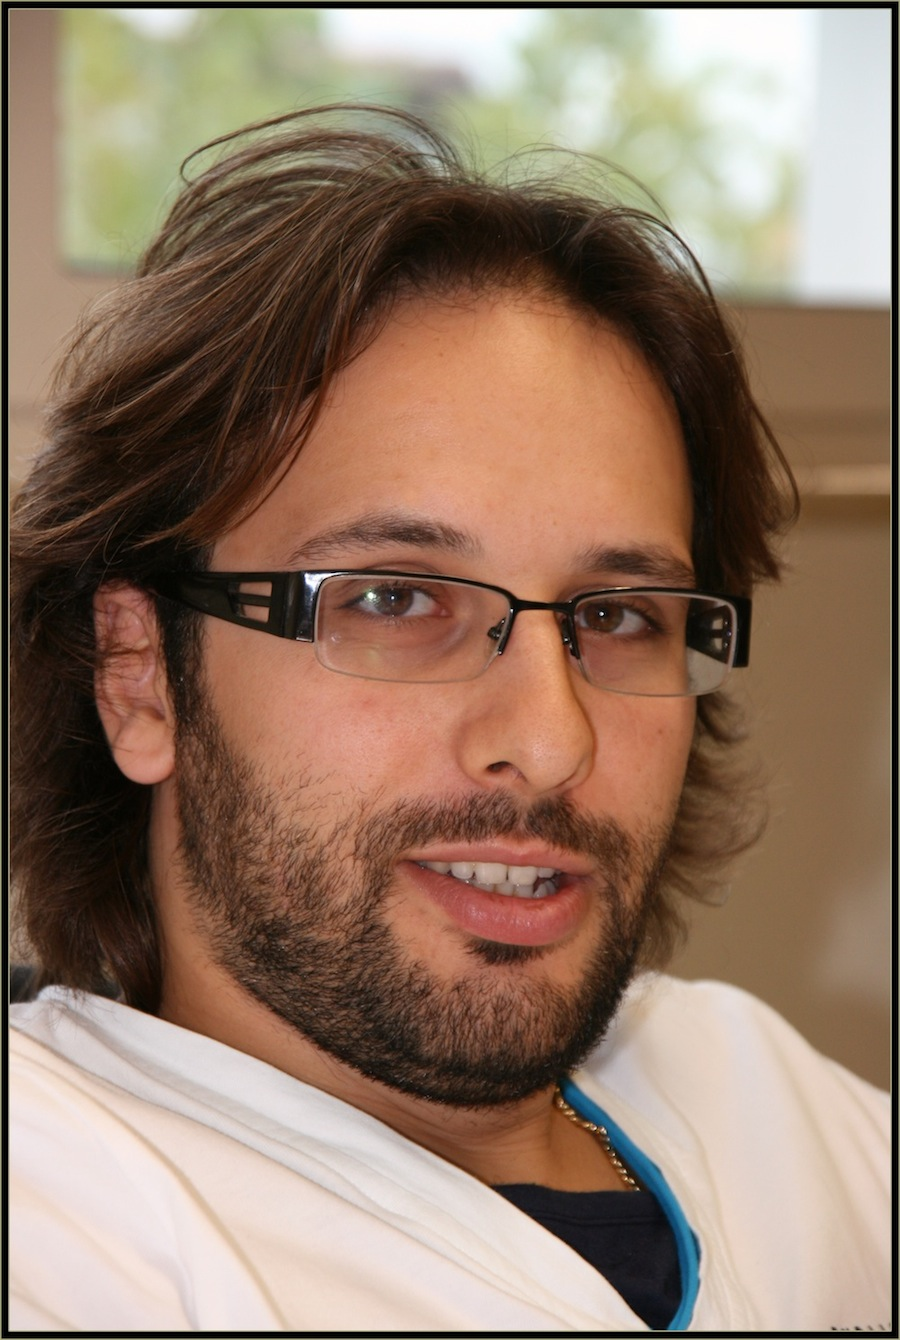
\includegraphics[width=10cm]{io.jpg}
            \end{center} 
        \end{figure}
        
    \end{center}
\pagebreak
\selectlanguage{english}

\begin{europecv}
\ecvpersonalinfo[5pt]

\ecvitem{\large\textbf{Desired employment / Occupational field}}{\large\textbf{I am looking for a position where I can express and use my passion for programming and technology. I mostly develop in Python/Django using OSX and Linux daily. Available for positions that give me personal and professional growth.}}

\ecvsection{Work experience}

\ecvitem{Dates}{\textbf{From April 26, 2008 to February 15, 2011}}
\ecvitem{Occupation or position held}{Programmer and System Engineer in \textbf{Research and Development} Department}
\ecvitem{Main activities and responsibilities}{Working in a research and development team to create of a innovative and unique product in the wireless communications market (WiFi), I initially worked on \textbf{embedded systems} (ubnt, alix, pcengines), customizing the operating system (ubnt, openwrt) and the softwares to manage authenitcation (hostapd, wpa-supplicant). After this first phase, I focused on the of software \textbf{to flash} these devices and on large-scale production software.

Also, we developed a complete solution for managing \textbf{hotspots}: I worked on server-side development to manage authentication, sessions log, signups, signals management from remote devices, integration with our management software, payment via credit card and authentication via SMS, complying with Pisanu law.
My final task was to create software for network monitoring. It is a \textbf{PyQT stand-alone} application, using internal django based API.

The technologies mostly used are Python/Django with PostgreSQL database on Debian OS virtualized on XEN}
\ecvitem{Name and address of employer}{Forinicom srl, Via del Popolo, 9 Bastia Umbra, 06083, 0758001868, \url{http://www.forinicom.it}}
\ecvitem[10pt]{Type of business or sector}{Telecommunication}

\ecvitem{Dates}{\textbf{From November 2010 to January 2011}}
\ecvitem{Occupation or position held}{\textbf{Python/Django} Programmer}
\ecvitem{Main activities and responsibilities}{Setting up an \textbf{Adult WebTV} entirely developed in Python/Django with PostgreSQL database on Linux/Apache platform and Red5 as streaming server. The work is managed independently using GIT as revision control system.}
\ecvitem{Name and address of employer}{Exion Telecom - Via Cantonale 2b - 6928 Manno, Switzerland, \url{http://www.exion.ch/}}
\ecvitem[10pt]{Type of business or sector}{IT solutions}

\ecvitem{Dates}{\textbf{From October 2010 to December 2010}}
\ecvitem{Occupation or position held}{\textbf{Python/Pylons} Programmer}
\ecvitem{Main activities and responsibilities}{Implementing new features, bug fixing, structural changes to the site of Sauce Labs. Distance work coordination site is developed in Python/Pylons using \url{github.com} as revision control system platform.}
\ecvitem{Name and address of employer}{Sauce Labs Inc - 500 Third St., San Francisco, CA 94107 USA, \url{http://saucelabs.com/}}
\ecvitem[10pt]{Type of business or sector}{Cross Browser Testing in the Cloud}

\ecvitem{Dates}{\textbf{From December 11, 2006 to August 31, 2008 and September 03, 2009 to December 31, 2010}}
\ecvitem{Occupation or position held}{\textbf{Python/Django} Programmer}
\ecvitem{Main activities and responsibilities}{Working in a team, I developed a management application for the municipality of Bettona using Django, Python, PostgreSQL, Linux, Apache, for the \textbf{computerization of services}, the management of personal data, building practices, urban planning, calculation of ICI tax and updating of land registry data. Also I created an advanced web interface for sending proposed practices, on-line services conference, integration process, exploration of cadastral map in \textbf{DXF} and production of customized an automated printing.

During the project I used revision control systems (SVN/GIT) with related web interface (trac) to manage tickets.}
\ecvitem{Name and address of employer}{Consorzio Miles - Servizi Integrati, CF 04881101002, Via Rocca di Papa 21, Rome \url{http://www.consorzio-miles.com/arianna/}}
\ecvitem[10pt]{Type of business or sector}{Integrated Services for Public Administration}

\ecvitem{Dates}{\textbf{From July 30, 2006 to December 30, 2006}}
\ecvitem{Occupation or position held}{Undergraduate student: Wireless Broadband Network - \textbf{Weconnect} project}
\ecvitem{Main activities and responsibilities}{The thesis was to develop a WiFi network in order to coverage \textbf{digital-divide} areas. Thanks to this project, I acquired a wide knowledge about WiFi networks and their behavior, legislation that governs the operation, RouterOS operating system (\url{www.mikrotik.com}), AAA protocol and Radius server. Finally I administered a server for the provision of various network services: mail (Postfix), web server (Apache), DNS (pdns), firewall (iptables), database (PostgreSQL), hotspot (Chillispot), Debian OS, Voyage (OS for embedded Debian based system).}
\ecvitem{Name and address of employer}{WEDOIT s.a.s. - Via Protomartiri Francescani,26 - 06088 Assisi (PG), \url{http://www.wedoit.us}}
\ecvitem[10pt]{Type of business or sector}{IT solutions}

\ecvitem{Dates}{\textbf{From 14 November 2005 to 30 May 2006}}
\ecvitem{Occupation or position held}{Trainee - \textbf{S.E.O. Search Engine Optimization}}
\ecvitem{Main activities and responsibilities}{Working in a team I acquired knowledge of S.E.O. and its behavior. The internship included S.E.O. optimization of various websites, using \emph{pagerank} and \emph{link popularity} methods. Also I worked as a system engineer of Debian-based virtualized server and I developed a S.E.O. oriented application in Python and PHP.}
\ecvitem{Name and address of employer}{WEDOIT s.a.s. - Via Protomartiri Francescani,26 - 06088 Assisi (PG), \url{http://www.wedoit.us}}
\ecvitem[10pt]{Type of business or sector}{IT solutions}

\ecvitem{Dates}{\textbf{March 2002}}
\ecvitem{Occupation or position held}{Trainee combined with IFS project, Impresa Formativa Simulata (Enterprise Training Simulation)}
\ecvitem{Main activities and responsibilities}{Administration of enterprise network}
\ecvitem{Name and address of employer}{IOSA CARLO S.r.l. - 05100 TERNI - Via Pallotta n. 7 - Tel. (0744) 2460 - Fax (0744) 246035 - P.IVA 00072550551 - \url{http://www.iosacarlo.com} - \url{iosacarlo@iosacarlo.com}}
\ecvitem[10pt]{Type of business or sector}{Waste disposal firm}

\ecvsection{Education and training}

\ecvitem{Dates}{\textbf{Since October 2008}}
\ecvitem{Title of qualification awarded}{Enrolled on course, with mayor in Computer Science, ``Security''}
\ecvitem{Principal subjects/occupational skills covered}{Passed following exams with mark:\begin{itemize}
    \item Simulation: 30 cum laude
    \item Advanced programming: 30 cum laude
    \item Advanced Operating Systems: 30 cum laude
    \item Advanced Operating Systems Laboratory: 30 cum laude
\end{itemize}}
\ecvitem{Name and type of organization providing education and training}{University of Perugia, Computer Science department, \url{http://informatica.unipg.it}}

\ecvitem{Dates}{\textbf{May 2010}}
\ecvitem{Title of qualification awarded}{\textbf{Diploma de Español como Lengua Extranjera} (D.E.L.E.) - Diploma in Spanish as a foreign language}
\ecvitem{Principal subjects/occupational skills covered}{The skills achieved are as follows:
\begin{itemize}
    \item reading comprension and written expression: 32.5 points out of 35.0
    \item grammar and vocabulary: 17.33 points out of 20
    \item comprehension and oral expression: 44.32 points out of 45
\end{itemize}}
\ecvitem{Name and type of organization providing education and training}{Instituto Cervantes, C/ Alcal\'a 49, E-28014 Madrid (Spagna), \url{http://www.cervantes.es}}
\ecvitem[10pt]{Level in national or international classification}{\textbf{B1 Level}\footnote{Evaluation according to ''Instituto Cervantes de Madrid''}}

\ecvitem{Dates}{\textbf{From October 14, 2009 to May 26, 2010}}
\ecvitem{Title of qualification awarded}{Certificates of attendance 42/50 hours of of the 3\superscript{rd} and 44/50 hours of the 4\superscript{th} modules of a Spanish language course}
\ecvitem{Principal subjects/occupational skills covered}{The skills achieved are as follows:
\begin{itemize}
    \item can understand the main points of clear standard speech on familiar matters
    \item able to describe experiences and events, reasons and projects
    \item can deal with most situations likely to arise whilst traveling in an area where the language is spoken
    \item understand sentences and frequently used expressions related to areas of most immediate relevance
    \item can describe in simple terms aspects of their history and own experiences
    \item can speak of the surrounding environment and be able to express needs, intentions and predictions
\end{itemize}}
\ecvitem{Name and type of organization providing education and training}{Comprehensive School ``Volumnio'' Ponte San Giovanni - Perugia}

\ecvitem{Dates}{\textbf{From August 2009 to March 2010}}
\ecvitem{Title of qualification awarded}{Paper publication \textbf{``The AES implementation based on OpenCL for multi/many core architecture''}}
\ecvitem{Principal subjects/occupational skills covered}{Preparation and publication of ``The AES implementation based on OpenCL for multi/many core architecture'' paper for the yearly conference ICCSA 2010 (\url{www.iccsa.org}) at Sangyo University, Fukuoka in Japan. The paper discuss the implementation of an AES algorithm that runs on NVIDIA/ATI graphics card.}
\ecvitem{Name and type of organization providing education and training}{University of Perugia, Computer Science department, \url{http://informatica.unipg.it}}

\ecvitem{Dates}{\textbf{From February 2007 to July 2007}}
\ecvitem{Title of qualification awarded}{Radio-amateur \textbf{class A license}}
\ecvitem{Principal subjects/occupational skills covered}{During the course for radio-amateur i acquired excellent knowledge of radio technology basics, radio devices and its usage and basics of Physics and Chemistry (magnetism, elettromagnetism)}
\ecvitem{Name and type of organization providing education and training}{C.I.S.A.R. Foligno's section}
\ecvitem[10pt]{Level in national or international classification}{PASSED, International Callsign \textbf{IZ0OVB}}

\ecvitem{Dates}{\textbf{From 19 March 2007 to 23 March 2007}}
\ecvitem{Title of qualification awarded}{Certificate of attendance, \textbf{Spanish course}}
\ecvitem{Principal subjects/occupational skills covered}{During the time in Madrid, I studied Spanish grammar and general Spanish culture.}
\ecvitem{Name and type of organization providing education and training}{Inhispania Intlance S.L / CIF:B83744847 , Montera 10-12, 1-1. 28013, Madrid (Spain)}
\ecvitem[10pt]{Level in national or international classification}{\textbf{A2\footnote{Evaluation according to ''Common European Framework of Reference for Languages''} Level}}

\ecvitem{Dates}{\textbf{01-02-03 Dicember 2006}}
\ecvitem{Title of qualification awarded}{Certificate of attendance: \textbf{ISO certifications course}}
\ecvitem{Principal subjects/occupational skills covered}{Training course on security and ISO certifications, covering ISO 27001:2005, policy for Information Security, Risks Analysis (RA), analysis of controls of ISO 17799:2005, Risk Transfer Process (RTP), certification process, overview of existing certification audits, audit plan and checklist, audit report, a look at future certifications.}
\ecvitem{Name and type of organization providing education and training}{WEDOIT s.a.s. - Via Protomartiri Francescani, 26 - 06088 Assisi (PG), Italy, \url{http://www.wedoit.us}}

\ecvitem{Dates}{\textbf{From October 2002 to November 2006}}
\ecvitem{Title of qualification awarded}{\textbf{Bachelor Degree in Computer Science}}
\ecvitem{Principal subjects/occupational skills covered}{Computer science Bachelor Degree, \textbf{mayor ``Network''}:
\begin{itemize}
    \item Mathematics (analytical and discrete)
    \item Programming (C, Java, Php, html, xml, xsl, dtd, Pascal, scripting bash and csh, VB.NET, VRML)
    \item Databases (Mysql, MS Access and related programming language)
    \item Networks (ATM, xDSL, Mpls, X.25, Frame Relay), types (wireless, wired) and interaction between them
    \item Knowledge of multimedia system
    \item Overview of parallel computing (mpi)
\end{itemize}}
\ecvitem{Name and type of organization providing education and training}{University of Perugia, Computer Science department, \url{http://informatica.unipg.it}}
\ecvitem[10pt]{Level in national or international classification}{\textbf{102/110}}

\ecvitem{Dates}{\textbf{From September 1996 to June 2002}}
\ecvitem{Title of qualification awarded}{\textbf{Accountant programmer Diploma (Mercurio project)}}
\ecvitem{Principal subjects/occupational skills covered}{Matters covered by the course (Commercial technical institute) of study as defined by the Ministry of Public Education: Chemistry / Physics, Mathematics and Computer Laboratory, Natural Science, Word processing and data, Second foreign language (French), Law and Economics, Business, Economics and Financial Science, Italian Language and Literature, History, Computer Management, Applied Mathematics, First foreign language (English), Law.}
\ecvitem{Name and type of organization providing education and training}{Ministry of Public Education - I.T.C. (Commercial technical institute) ``Federico Cesi'', Terni (TR), Italy}
\ecvitem[10pt]{Level in national or international classification}{\textbf{85/100}}

\ecvitem{Dates}{\textbf{From 2001 to 2002}}
\ecvitem{Title of qualification awarded}{Certificate of attendance of the National Project IFS (\textbf{Enterprise Training Simulation})}
\ecvitem{Principal subjects/occupational skills covered}{Simulation of waste disposal firm, backed by Iosa Carlo S.r.l. (\url{http://www.iosacarlo.com}).
Within the project I coordinated the work of all students, building the simulated organization chart and programming the website.}
\ecvitem{Name and type of organization providing education and training}{Ministry of Public Education - I.T.C. (Commercial technical institute) ``Federico Cesi'', Terni (TR), Italy}

\ecvsection{Personal skills and competences}

\ecvmothertongue[5pt]{Italian}
\ecvitem{\large Other language(s)}{\textbf{English, Spanish}}
\ecvlanguageheader{(*)}
\ecvlanguage{English}{\ecvBOne}{\ecvBOne}{\ecvATwo\ecvBOne}{\ecvATwo\ecvBOne}{\ecvBOne}
\ecvlastlanguage{Spanish}{\ecvBOne}{\ecvBOne}{\ecvBOne}{\ecvBOne}{\ecvBOne}
\ecvlanguagefooter[10pt]{(*)}

\ecvitem[10pt]{Social skills and competences}{Working usually in a team, I have a constructive and collaborative relationship with the people around me, such as colleagues and collaborators. I am sociable, friendly and with good communication skills; my site is a source of continuing social contact and exchange with other technical and less technical people.}
\ecvitem[10pt]{Organizational skills and competences}{Determenated, I can work both in a team and individually. I am able to manage independently my workflow.}
\ecvitem[10pt]{Computer skills and competences}{Because of \textbf{my passion for computing}, I have developed over the years wide range of skills many areas computer-related.

Durint the years of higher education, beyond academic success, I created and maintained an \textbf{above average} extra-crricular activity: among other initiatives in which I participated, I remember ''The basic course on multimedia'',''Exposcuola 2000 in Paestum'', ''Basic computer as tutor role'', ''Computer literacy course as tutor to senior people (over 65 years old)'', ''XI week of scientific and technological culture'', ''Pluto Meeting 2001'' and ''Main tutor of a group of 6 people for the course of IMPROVING ITALIAN for new students in the project ''Reception, Recovery, Empowerment in early grades''''. In all the projects mentioned, I participated actively devoting time and effort in learning new things about new information technology and other subjects.

From the moment I had my first computer, I have had a certain passion for the \textbf{open source} world and all that concerns it: in fact I have managed machines with \textbf{Linux} distributions such as RedHat 7.3, Slackware 7.1 up to machines to Debian (from version 3.0 to current ones). Through this experience I have gained skill and knowledge in the management of Linux: bash scripting, configuring and compiling the kernel, network services, patching the kernel, C language. In addition to Linux, I daily use OSX. Given the continued use and my passion for computers, I have undertaken in-depth study of the latter.

I was active as a contributor to the writing of the guide \url{http://www.ubuntusemplice.org/} (version 6.06 and 7.10). On this project I was the reviewer and author of several chapters, I administered the machine that hosts the site, wiki, blog and mailing list.

\textbf{I also have a great passion for programming languages}: I know many of them in several areas such as Python, C, PHP, Java, LSL (Linden Scripting Language). I studied LSL during my work on \textbf{Second Life}: in fact I have worked on many Italian metaverse project such as Assis \url{http://www.secundavita.it}, Milan and Marostica on the \textbf{''Italia Vera''} project.
I have a good knowledge of graphic applications (Gimp, Photoshop) and office tools such as Openoffice.org and iWork (for OSX)}
\ecvitem[10pt]{Artistic skills and competences}{\vspace{-2mm}
\begin{itemize}
    \item Learning the Spanish language by myself
    \item Amateur photos
    \item Music (hobby level)
\end{itemize}}

\ecvitem[10pt]{Other skills and competences}{\vspace{-2mm}
\begin{itemize}
    \item Curious by definition
    \item Music
    \item Willing to learn and study
    \item Attraction for science in general
\end{itemize}}

\ecvitem{Licence(s)}{\vspace{-2mm}
\begin{itemize}
    \item Driving license type B.
    \item Operator license for amateur radio station class A (nr. 020122/AN), International callsign \textbf{IZ0OVB}
\end{itemize}}

\ecvsection{Additional information}

\ecvitem[10pt]{}{\vspace{-10mm}
\begin{itemize}
    \item comply with compulsory military service (referring to studies)
    \item Linux Registered User \#399008
    \item ordinary member of the LUG Perugia
    \item AVIS (Blood Donor Italian Association) ordinary member
    \item marital status: single
\end{itemize}}

\ecvsection{Attachment}
\ecvitem{}{No attachments}

\end{europecv}
\end{document} 